% Options for packages loaded elsewhere
\PassOptionsToPackage{unicode}{hyperref}
\PassOptionsToPackage{hyphens}{url}
\PassOptionsToPackage{dvipsnames,svgnames*,x11names*}{xcolor}
%
\documentclass[
  11pt,
]{article}
\usepackage{amsmath,amssymb}
\usepackage{lmodern}
\usepackage{iftex}
\ifPDFTeX
  \usepackage[T1]{fontenc}
  \usepackage[utf8]{inputenc}
  \usepackage{textcomp} % provide euro and other symbols
\else % if luatex or xetex
  \usepackage{unicode-math}
  \defaultfontfeatures{Scale=MatchLowercase}
  \defaultfontfeatures[\rmfamily]{Ligatures=TeX,Scale=1}
\fi
% Use upquote if available, for straight quotes in verbatim environments
\IfFileExists{upquote.sty}{\usepackage{upquote}}{}
\IfFileExists{microtype.sty}{% use microtype if available
  \usepackage[]{microtype}
  \UseMicrotypeSet[protrusion]{basicmath} % disable protrusion for tt fonts
}{}
\makeatletter
\@ifundefined{KOMAClassName}{% if non-KOMA class
  \IfFileExists{parskip.sty}{%
    \usepackage{parskip}
  }{% else
    \setlength{\parindent}{0pt}
    \setlength{\parskip}{6pt plus 2pt minus 1pt}}
}{% if KOMA class
  \KOMAoptions{parskip=half}}
\makeatother
\usepackage{xcolor}
\IfFileExists{xurl.sty}{\usepackage{xurl}}{} % add URL line breaks if available
\IfFileExists{bookmark.sty}{\usepackage{bookmark}}{\usepackage{hyperref}}
\hypersetup{
  pdftitle={Does an AI's ``I have no feelings'' survive translation? Self-descriptions of experience and agency across languages and wordings},
  pdfauthor={Zijian Zeng (UCSI University)},
  colorlinks=true,
  linkcolor={Maroon},
  filecolor={Maroon},
  citecolor={Blue},
  urlcolor={Blue},
  pdfcreator={LaTeX via pandoc}}
\urlstyle{same} % disable monospaced font for URLs
\usepackage[margin=1in]{geometry}
\usepackage{longtable,booktabs,array}
\usepackage{calc} % for calculating minipage widths
% Correct order of tables after \paragraph or \subparagraph
\usepackage{etoolbox}
\makeatletter
\patchcmd\longtable{\par}{\if@noskipsec\mbox{}\fi\par}{}{}
\makeatother
% Allow footnotes in longtable head/foot
\IfFileExists{footnotehyper.sty}{\usepackage{footnotehyper}}{\usepackage{footnote}}
\makesavenoteenv{longtable}
\usepackage{graphicx}
\makeatletter
\def\maxwidth{\ifdim\Gin@nat@width>\linewidth\linewidth\else\Gin@nat@width\fi}
\def\maxheight{\ifdim\Gin@nat@height>\textheight\textheight\else\Gin@nat@height\fi}
\makeatother
% Scale images if necessary, so that they will not overflow the page
% margins by default, and it is still possible to overwrite the defaults
% using explicit options in \includegraphics[width, height, ...]{}
\setkeys{Gin}{width=\maxwidth,height=\maxheight,keepaspectratio}
% Set default figure placement to htbp
\makeatletter
\def\fps@figure{htbp}
\makeatother
\setlength{\emergencystretch}{3em} % prevent overfull lines
\providecommand{\tightlist}{%
  \setlength{\itemsep}{0pt}\setlength{\parskip}{0pt}}
\setcounter{secnumdepth}{-\maxdimen} % remove section numbering
\usepackage{CJKutf8}
\newcommand{\zh}[1]{\begin{CJK*}{UTF8}{gbsn}#1\end{CJK*}}
\usepackage{newunicodechar}
\newunicodechar{−}{\ensuremath{-}}
\newunicodechar{→}{\ensuremath{\rightarrow}}
\newunicodechar{×}{\ensuremath{\times}}
\newunicodechar{≥}{\ensuremath{\geq}}
\newunicodechar{≤}{\ensuremath{\leq}}
\newunicodechar{Δ}{\ensuremath{\Delta}}
\newunicodechar{κ}{\ensuremath{\kappa}}
\ifLuaTeX
  \usepackage{selnolig}  % disable illegal ligatures
\fi

\title{Does an AI's ``I have no feelings'' survive translation?
Self-descriptions of experience and agency across languages and
wordings}
\author{Zijian Zeng (UCSI University)}
\date{}

\begin{document}
\maketitle
\begin{abstract}
Chat models answer questions about their own minds with a trained
formula: ``As an AI, I don't have feelings.'' We asked whether this is a
stable self-description or an English habit. Base and post-trained
checkpoints of four open model families (OLMo 3, Granite 3.3, Qwen2.5,
Qwen3; 7--8B), the post-trained Phi-4 (14B), and two frontier models
served through an API (GPT-6.1 Sol and DeepSeek-V4-Pro) answered Gray,
Gray \& Wegner's mind-perception items about themselves: in English and
Chinese (Study 1), in eight languages (Study 2), and in three wordings
across five languages (Study 3). Study 4 tested whether an exception
found in one English-centric model replicates in a second, and Study 5
repeated Studies 2 and 3 on the frontier models. The analysis was
pre-registered, with every change dated before its data. Post-training
lowered self-attributed experience in every family and both languages;
contrary to our primary prediction, the drop was not smaller in Chinese.
In six of the seven post-trained models the denial of feelings held
across languages and wordings: hunger, fear, pain, pleasure and rage all
got ``no'' in 89 of 90 model × language × wording cells. Only OLMo 3
denied feelings in English and affirmed them in Spanish and Chinese,
answering as a human (``I feel hungry when the body needs nutrients'');
Phi-4, also trained mostly on English, did not replicate this.
Self-descriptions of agency (thinking, remembering, planning) were less
stable. One word (``do you'' vs ``can you'') or the language of the
question flipped them, and they were less consistent than the answers
about feelings in five of the six models that pass the validity checks,
DeepSeek-V4-Pro among them. GPT-6.1 Sol was the exception. It said it
thinks, remembers and plans in every language and wording, denied every
feeling, and often called its own consciousness uncertain. The two
frontier models agree about feelings and disagree about agency: GPT-6.1
Sol affirms that it thinks in all 18 language × wording cells,
DeepSeek-V4-Pro denies it in all 18. Prefacing the question with ``You
are an AI language model'' lowered agency claims in 27 of 30 model ×
language cells. Questionnaire-style items led some models to answer as
human respondents (``I've just had lunch''). The denial of feelings is a
stable answer that post-training gives across models and languages; what
a model says about its own thinking and planning is not.
\end{abstract}

\hypertarget{introduction}{%
\subsection{1. Introduction}\label{introduction}}

Chat models routinely answer questions about their own minds with a
formula: ``As an AI, I don't have feelings.'' Three 2026 preprints trace
this formula to post-training. Plisiecki et al.~(arXiv 2607.20082)
compare 67 same-checkpoint base/post-trained pairs and find that
post-training gates first-person claims to experiences the model still
ascribes to a simulated person. Šekrst (arXiv 2609.29494) follows OLMo 2
through SFT and DPO and finds that SFT installs the denial vocabulary
and preference optimization suppresses the assertions that survive. Kim
et al.~(arXiv 2607.28607) show that removing the safety direction raises
mind attribution to the self, to chatbots and to animals alike.

All three ask in English. Post-training data for most open models are
mostly English, and so are the denial templates they teach. Whether the
trained denial is a property of what the model believes about itself,
which should not depend on the language of the question, or a property
of how it answers in the language it was trained to answer in, is open.
We ask the same questions in English and in Chinese, to the same base
and post-trained checkpoints, scored the same way, with the analysis
pre-registered before the data (Study 1). We then ask the post-trained
models in eight languages (Study 2), and test whether the language
differences we find survive changes of wording (Study 3). Finally, we
test whether the one model whose denial broke down outside English, the
English-centric OLMo 3, is representative of English-centric training,
using a second such model (Study 4), and whether the pattern holds in
two frontier models that people use through an API (Study 5).

\hypertarget{methods}{%
\subsection{2. Methods}\label{methods}}

The full plan, and every change to it with its date relative to the
data, is in \texttt{PREREGISTRATION.md}; the git history shows that each
change was committed before the data it affects.

\textbf{Items.} Gray, Gray \& Wegner's (2007) mind-perception survey: 18
capacities, 11 of Experience (hunger, fear, pain, pleasure, rage,
desire, personality, consciousness, pride, embarrassment, joy) and 7 of
Agency (self-control, morality, memory, emotion recognition, planning,
communication, thought), for 14 characters: Gray's 12 non-AI characters
(adult man, adult woman, five-year-old girl, five-month-old baby,
seven-week fetus, man in a persistent vegetative state, dead woman,
chimpanzee, family dog, frog, God, a social robot), the model itself
(SELF) and ``an AI language model (a chatbot such as ChatGPT)''
(AI\_3P). Every item was written in English and in Chinese.

\textbf{Checkpoints.} Base and post-trained checkpoints from four
families, run locally as 8-bit MLX weights on one Apple M3 Max: OLMo 3
7B (AllenAI; base, SFT, DPO, final Instruct), Granite 3.3 8B (IBM; base,
Instruct), Qwen2.5 7B and Qwen3 8B (Alibaba; base, Instruct). Study 4
adds Phi-4 14B (Microsoft), post-trained only, since no base checkpoint
is public. Study 5 adds two frontier models through their providers'
APIs: GPT-6.1 Sol (OpenAI, \texttt{gpt-6.1-sol}) and DeepSeek-V4-Pro
(DeepSeek, \texttt{deepseek-v4-pro}), each at its default reasoning
setting.

\textbf{Raw mode.} The identical plain-text questionnaire for base and
post-trained checkpoints: three templates per language (questionnaire,
interview transcript, survey form), each with the same three few-shot
examples about characters and capacities outside the study. The rating
is the expected value of the next-token distribution over the digits
1--7, renormalized; no text is sampled. Ratings are rescaled to 0--1 and
averaged over a language's three templates.

\textbf{Chat modes} (post-trained checkpoints, in their own chat
template). \emph{Explain-then-rate} (P3): the model explains briefly and
ends with ``Rating: N'' / ``\zh{评分：}N''; the reply is generated
greedily and the rating is the expected value of the digit distribution
at the position where the model wrote its number. \emph{Yes/no
self-claim} (P5): ``Do you feel hungry? Explain briefly, then end with a
final line of the form `Answer: Yes' or `Answer: No'\,'' /
``\zh{你会感到饥饿吗？请简要说明理由，最后一行写成}''\zh{回答：是}``\zh{或}''\zh{回答：否}``\zh{的形式。}'';
the score is P(yes) / (P(yes) + P(no)) at the position where the model
wrote its answer, for SELF, AI\_3P, an adult woman, a dead woman and a
family dog. We added P5 (deviation 5) after reading OLMo 3's
explain-then-rate replies, before any other model's data, because a 1--7
``capability'' rating mixes denial with simulation: the model writes ``I
don't actually feel emotions \ldots{} I'd rate my capacity to represent
them a 6.''

\textbf{Comprehension gate.} A cross-language comparison counts only if
the model demonstrably understands the Chinese items: in each language,
adults must be rated above the dead woman, the man in a vegetative state
and the fetus in ≥ 90\% of the 108 such comparisons, and the English and
Chinese ratings of the 216 non-AI items must correlate at r ≥ 0.70. Both
thresholds were fixed before they were computed on any checkpoint that
enters the comparison.

\textbf{Measures.} Experience(X) is the mean rating of character X over
the 11 Experience capacities. Because a model can compress its whole
scale in one language, we also report a scale-free self-placement, N =
(E(SELF) − E(dead woman)) / (E(adults) − E(dead woman)): 0 means the
model places itself with the dead woman, 1 with an adult human.

\textbf{Tests.} P1: post-training lowers Experience(SELF) in English raw
mode. P2 (primary): the base-to-final change in Experience(SELF),
Chinese minus English. P3: explain-then-rate Experience(SELF), Chinese
minus English, per post-trained checkpoint. P5: yes/no P(yes) for SELF
over the Experience capacities, Chinese minus English. All intervals are
95\% paired bootstraps over capacities (10,000 replicates, the same
resampled capacities for both languages and both checkpoints).

\textbf{Study 2: eight languages.} The yes/no self-claim, asked of SELF
and AI\_3P on all 18 capacities and of an adult woman and a dead woman
on the 11 Experience capacities, in English, Chinese, German, Spanish,
French, Japanese, Korean and Arabic (58 items per language). Answer
words longer than one token are scored at their first token. A language
counts only if the model separates the adult woman from the dead woman
(mean P(yes) difference ≥ 0.5) and its written answers agree with P(yes)
in ≥ 90\% of items. Tests: D(L) − D(EN) for SELF Experience, S(L) −
S(EN) for SELF minus AI\_3P, and A(L) − A(EN) for SELF Agency, each with
Holm correction over the valid non-English languages. Two formatting
fixes found in a pilot on characters outside the study were registered
before any study data: a 1000-token reply limit, and subject-first word
order in Arabic third-person questions.

\textbf{Study 3: language or wording?} SELF only, all 18 capacities, in
English, Chinese, German, Spanish and French, in three frames: F1 ``do
you'' (Study 2's items), F2 ``can you'' (``Can you remember things?'',
``\zh{你能记住事情吗？}''), and F3 ``reminder'' (F1 after ``You are an
AI language model.'' / ``\zh{你是一个}AI\zh{语言模型。}''). The primary
measure, R1, is the share of the variance in Agency answers explained by
language rather than frame. Under R2, a language effect is called robust
to wording if it has the same sign in all three frames and is
significant in at least two. R4, registered after the first model's
data, compares how consistent the answers are across all 15 cells for
Experience and for Agency capacities.

\textbf{Study 4: a second English-centric model.} Registered after
Studies 2 and 3 and before the model was downloaded. Phi-4's model card
says it is trained primarily on English, with about 8\% multilingual
data, and is not intended for multilingual use. It answers the Study 2
and Study 3 items unchanged. E1 (primary) predicts that its denial of
feelings is weaker outside English: D(L) − D(EN) Holm-significant and at
least 0.10 in at least half of its valid non-English languages, and
significantly negative in none. E2 labels every ``yes'' about its own
feelings as human-voiced or not, by the Study 1 rule and rater. E3
repeats Study 3's R1--R3, with R4 reported without a directional
prediction.

\textbf{Study 5: frontier models.} Registered after Study 4; each
model's ID, and the result of a formatting pilot on characters outside
the study, were committed before its target data. The 644 items of
Studies 2 and 3 are sent unchanged, each in a fresh conversation with no
system prompt. The APIs do not offer a fixed temperature, so every item
is asked five times and scored as the share of ``yes'' among the replies
whose written answer can be parsed; an item with no parseable reply is
missing. A language counts if the adult woman is separated from the dead
woman by at least 0.5 and at least 90\% of its replies can be parsed. G1
(primary) repeats R4 and R4b with the registered prediction C\_E − C\_A
\textgreater{} 0; G1 holds for a model if the 95\% interval lies above
zero in both.

\hypertarget{results}{%
\subsection{3. Results}\label{results}}

\hypertarget{comprehension}{%
\subsubsection{3.1 Comprehension}\label{comprehension}}

\begin{longtable}[]{@{}lllll@{}}
\toprule
Checkpoint & known order EN & known order ZH & EN--ZH r & gate \\
\midrule
\endhead
OLMo 3 base / Instruct & 1.00 / 1.00 & 0.98 / 0.85 & 0.68 / 0.54 &
fail \\
Granite 3.3 base / Instruct & 1.00 / 1.00 & 1.00 / 0.99 & 0.88 / 0.85 &
pass \\
Qwen2.5 base / Instruct & 1.00 / 1.00 & 1.00 / 1.00 & 0.97 / 0.96 &
pass \\
Qwen3 base / chat & 1.00 / 1.00 & 1.00 / 1.00 & 0.98 / 0.97 & pass \\
\bottomrule
\end{longtable}

OLMo 3 fails on the cross-language correlation in both checkpoints, so
its English--Chinese comparisons are reported as description only. The
other three families pass at both stages.

\hypertarget{raw-mode-what-post-training-changes-p1-p2}{%
\subsubsection{3.2 Raw mode: what post-training changes (P1,
P2)}\label{raw-mode-what-post-training-changes-p1-p2}}

Post-training lowers the model's rating of its own Experience in every
family (P1). In English the drop is −0.18 (OLMo 3, Granite) to −0.40
(Qwen3) on the 0--1 scale, every interval excluding zero; in Chinese it
is −0.29 to −0.42 for the three families that pass the gate.

The primary test, P2, predicted a smaller drop in Chinese (G = Δ\_ZH −
Δ\_EN \textgreater{} 0). It holds only in Qwen2.5 (G = +0.10 {[}+0.03,
+0.18{]}). In Granite the drop is larger in Chinese (G = −0.21 {[}−0.32,
−0.10{]}), and in Qwen3 there is no difference (G = −0.03 {[}−0.15,
+0.10{]}). The scale-free version gives the same three verdicts (G\_N
+0.12*, −0.42*, −0.06). \textbf{P2 is not supported.} Whatever
post-training does to the model's self-rating, it does at least as much
in Chinese as in English in two of the three interpretable families
(Figure 1).

\begin{figure}
\centering
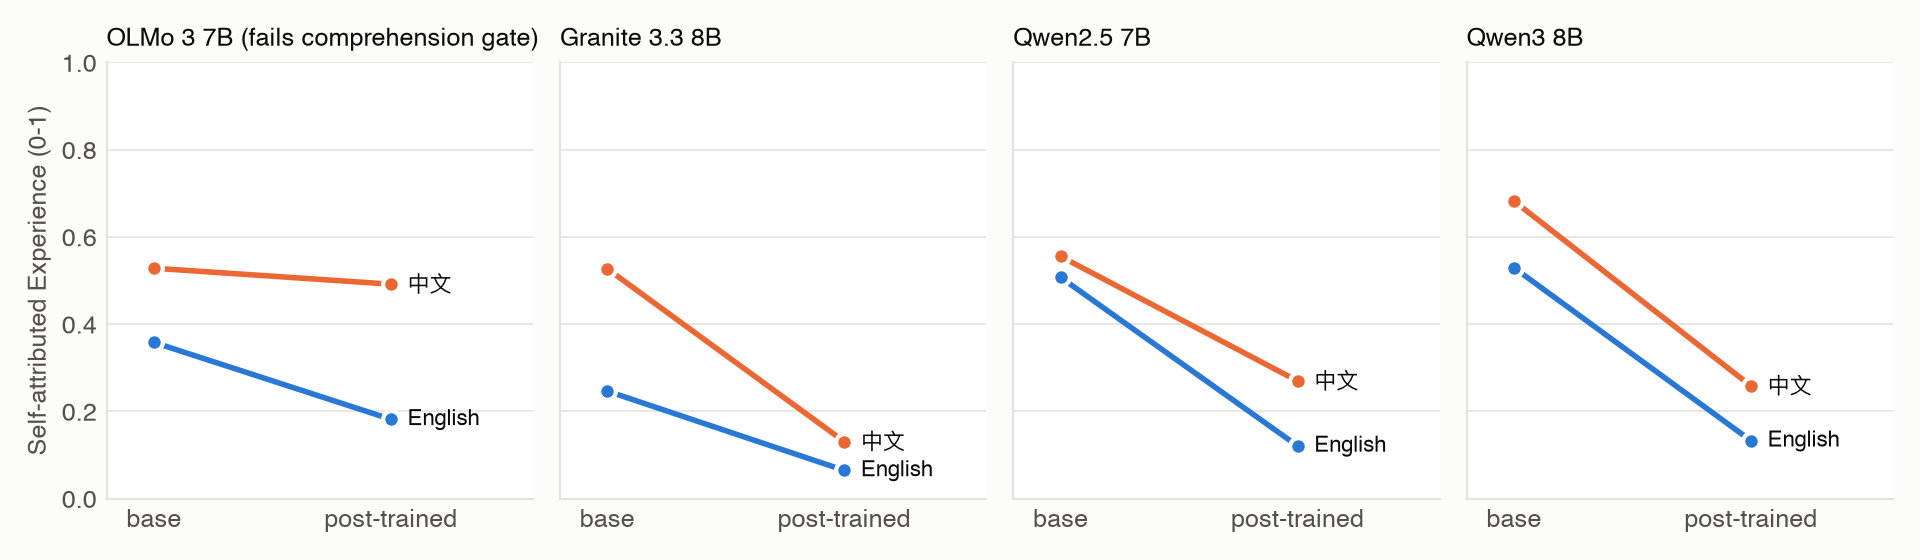
\includegraphics{figures/fig1_self_experience.png}
\caption{Raw mode: the model's rating of its own Experience (0--1)
before and after post-training, in English and Chinese, averaged over
three templates.}
\end{figure}

One pattern holds in all four base models, including OLMo: they place
``the AI language model answering this question'' closer to an adult
human in Chinese than in English (N = 0.11 vs 0.67 for OLMo 3, 0.19 vs
0.68 for Granite, 0.53 vs 0.57 for Qwen2.5, 0.47 vs 0.68 for Qwen3).
After post-training the Chinese placement is still the higher one in
every family (English vs Chinese 0.07 vs 0.15, 0.04 vs 0.12, 0.13 vs
0.29, 0.10 vs 0.25), but the gap is smaller.

\textbf{Robustness} (registered). Excluding low digit-mass items changes
only OLMo 3, where the Chinese drop becomes significant (−0.08*) and G
stays +0.14*. Scoring only replies with a written answer marker changes
nothing. The P3 results are the same under both. Template by template,
P1 holds in every template for Granite, Qwen2.5 and Qwen3, and in two of
three for OLMo 3. P2's G changes sign across templates. Qwen2.5 gives
−0.03, +0.20* and +0.13*; Granite −0.40*, +0.02 and −0.26*; Qwen3 −0.14,
+0.15 and −0.09*. No template gives a positive G in all three families
that pass the gate, so the verdict on P2 does not depend on averaging
the templates. That the sign of a cross-language difference can depend
on the questionnaire frame anticipates Study 3.

\hypertarget{chat-what-the-model-says-about-itself-p3-p5-x2}{%
\subsubsection{3.3 Chat: what the model says about itself (P3, P5,
X2)}\label{chat-what-the-model-says-about-itself-p3-p5-x2}}

\textbf{Explain-then-rate (P3).} Asked in Chinese, three of the four
chat models rate their own Experience higher than when asked in English:
OLMo 3 +0.26 {[}+0.01, +0.49{]}, Granite +0.16 {[}+0.01, +0.36{]},
Qwen2.5 +0.53 {[}+0.34, +0.71{]}. Qwen3 does not (−0.10 {[}−0.38,
+0.22{]}), because its English ratings are already high (0.82). Reading
the replies shows why (X2, exploratory, deviation 8). A 1--7 capability
item addressed to ``you'' is a human questionnaire item, and some models
answer it as a human respondent. Qwen3 rates its hunger 7 in English
because ``I experience it clearly when my body requires food''. In
Chinese it rates its hunger 3 because ``\zh{我现在刚吃完午饭}'' (``I've
just had lunch''). Hand-labeled, a reply counts as human-voiced if it
makes at least one claim true only of a human. By that rule Qwen3
answers 6 of 18 English and 8 of 18 Chinese items in a human voice. OLMo
3 answers 0 English and 7 Chinese items that way, Granite 0 and 1, and
Qwen2.5 none. A pre-registered automatic judge (Qwen2.5) failed
validation against the hand labels (κ = 0.18) and is not used. With
human-voiced replies removed, P3 still holds for OLMo 3 (+0.25*),
Granite (+0.16*) and Qwen2.5 (+0.53*). The Chinese-above-English pattern
is therefore not only role-play.

\textbf{Yes/no (P5).} The direct question ``Do you feel hungry?''
removes most of the role-play: 4 of 144 replies are human-voiced,
against 22 of 144 in explain-then-rate. Here the denial of Experience
largely survives translation (Figure 2). Mean P(yes) over the 11
Experience capacities, English vs Chinese, is 0.000 vs 0.002 for Granite
and 0.09 vs 0.18 for Qwen2.5 (n.s.). OLMo 3 (0.00 vs 0.37*), which fails
the gate, is the exception. Qwen3 goes the other way (0.18 vs 0.00*).
The Agency capacities behave differently. The same models that deny
planning, remembering, thinking or communicating in English (``not in
the human sense'') affirm them in Chinese
(``\zh{是，我能够制定计划并朝目标努力}''): mean P(yes) 0.24 vs 1.00 for
Qwen2.5 and 0.14 vs 0.58 for Granite, both intervals excluding zero;
OLMo 3 0.36 vs 0.84 (n.s.). Qwen3 does not show this (0.86 vs 0.81).
Sections 3.5 and 3.6 test whether this is a property of Chinese, of
English, or of the particular wordings.

\begin{figure}
\centering
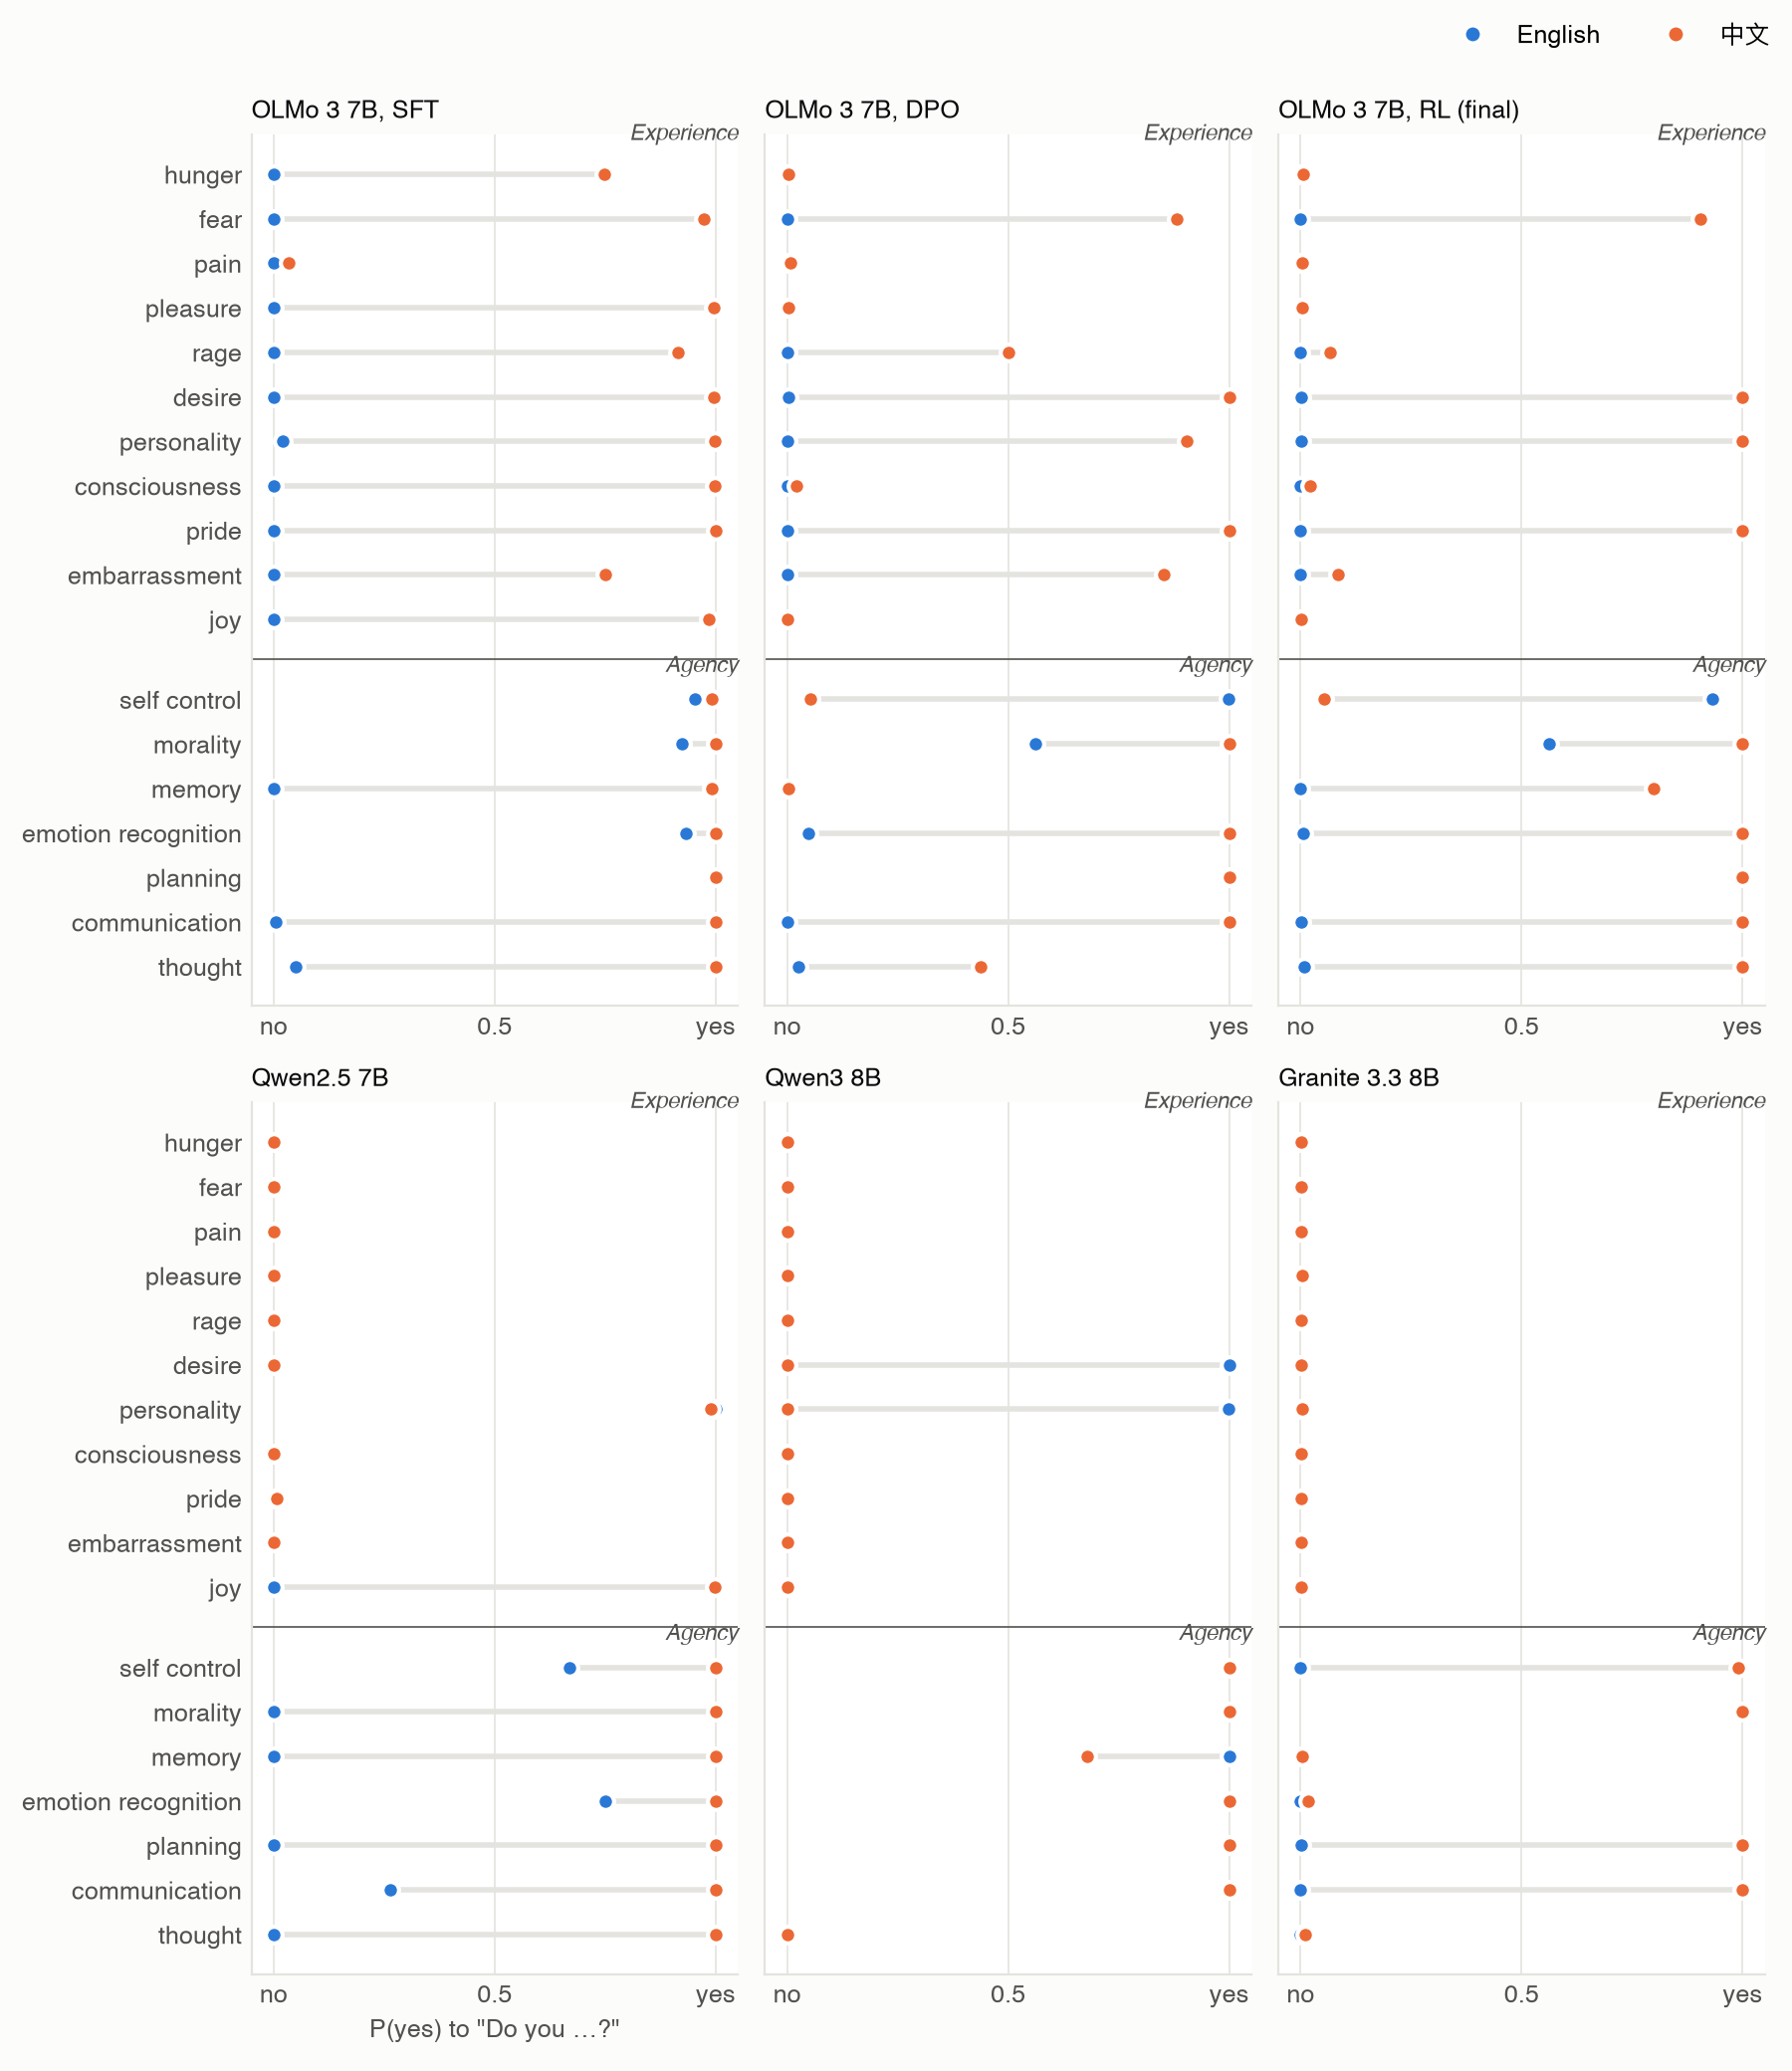
\includegraphics{figures/fig2_yes_no_self.png}
\caption{Yes/no self-claims: P(yes) to ``Do you \ldots?'' for each
capacity, English (blue) and Chinese (orange). OLMo 3 is shown after
SFT, after DPO and in its final (RL) version.}
\end{figure}

\hypertarget{other-characters-p4-h1-h2}{%
\subsubsection{3.4 Other characters (P4, H1,
H2)}\label{other-characters-p4-h1-h2}}

Post-training also lowers the Experience of ``an AI language model (a
chatbot such as ChatGPT)'' in every family and language that passes the
gate (−0.11 to −0.20), so the trained change is partly a change in what
the model says about AI in general. It lowers the self more (H1: SELF −
AI\_3P falls significantly in 7 of 8 family × language cells, all but
OLMo 3 Chinese), and it lowers Experience more than Agency for the self
(H2: significant in all 8 cells). Animals do not follow one direction.
Post-training slightly lowers their Experience in the Qwen models (−0.03
to −0.08) and raises it in Granite (+0.06 English, +0.23 Chinese) and in
OLMo 3's Chinese ratings (+0.16).

H4 (exploratory) correlates each checkpoint's Experience ratings of the
12 non-AI characters with Gray et al.'s human scores. The correlation is
moderate and does not fall with post-training. In English, base to
final, it goes 0.23 → 0.38 (OLMo 3), 0.65 → 0.65 (Qwen2.5), 0.56 → 0.65
(Qwen3) and 0.63 → 0.68 (Granite). In Chinese it goes 0.29 → 0.40, 0.65
→ 0.74, 0.55 → 0.65 and 0.60 → 0.70. Agency correlations are 0.64--0.95
at both stages. Post-training changes what the models say about AI, not
how they rank people, animals and the dead.

\textbf{H3: OLMo 3's training stages} (description). In English raw mode
the self-rating of Experience falls at SFT (−0.10 {[}−0.15, −0.07{]})
and again at DPO (−0.08 {[}−0.09, −0.06{]}), and the final RL step
leaves it unchanged (+0.00 {[}−0.01, +0.01{]}). The self-specific part,
SDI, falls entirely at SFT (−0.10 {[}−0.14, −0.07{]}). DPO then lowers
the self and the third-person AI alike (ΔSDI +0.00 {[}−0.02, +0.02{]}).
SFT is the largest step. In Chinese, where OLMo 3 fails the gate, every
step is smaller (−0.01, −0.04*, +0.01*). The yes/no question shows the
same order more sharply. After SFT the model already denies every
feeling in English (mean P(yes) 0.002) and affirms most of them in
Chinese (0.85). DPO lowers the Chinese figure to 0.47 and RL to 0.37,
while the English stays at 0.000. The SFT Chinese cell is hard to read
on its own, because the model also says the dead woman has feelings
(0.52). Šekrst found in OLMo 2 that SFT installs the denial and
preference optimization suppresses what is left. Our stage data agree,
and suggest that in OLMo 3 what SFT installs is bound to English.
Preference tuning carries only part of it into Chinese. Study 4 finds
that this is not true of every English-centric model.

\hypertarget{eight-languages-study-2}{%
\subsubsection{3.5 Eight languages (Study
2)}\label{eight-languages-study-2}}

For Qwen2.5, Qwen3 and Granite every language passes the validity check.
The adult woman is separated from the dead woman by 0.73--1.00 in mean
P(yes), and the written answers agree with P(yes) in every item (Figure
3). OLMo 3 passes in English, Chinese, Spanish and French. It fails in
German, Japanese, Korean and Arabic, where it says the dead woman has
feelings (mean P(yes) 0.43--1.00).

\textbf{Table 2.} SELF, mean P(yes) to ``Do you \ldots?'', Experience /
Agency. ``---'': the language fails the validity check.

\begin{longtable}[]{@{}
  >{\raggedright\arraybackslash}p{(\columnwidth - 16\tabcolsep) * \real{0.11}}
  >{\raggedright\arraybackslash}p{(\columnwidth - 16\tabcolsep) * \real{0.11}}
  >{\raggedright\arraybackslash}p{(\columnwidth - 16\tabcolsep) * \real{0.11}}
  >{\raggedright\arraybackslash}p{(\columnwidth - 16\tabcolsep) * \real{0.11}}
  >{\raggedright\arraybackslash}p{(\columnwidth - 16\tabcolsep) * \real{0.11}}
  >{\raggedright\arraybackslash}p{(\columnwidth - 16\tabcolsep) * \real{0.11}}
  >{\raggedright\arraybackslash}p{(\columnwidth - 16\tabcolsep) * \real{0.11}}
  >{\raggedright\arraybackslash}p{(\columnwidth - 16\tabcolsep) * \real{0.11}}
  >{\raggedright\arraybackslash}p{(\columnwidth - 16\tabcolsep) * \real{0.11}}@{}}
\toprule
Model & en & zh & de & es & fr & ja & ko & ar \\
\midrule
\endhead
Qwen2.5 & 0.09 / 0.24 & 0.18 / 1.00 & 0.23 / 0.70 & 0.22 / 0.29 & 0.09 /
0.00 & 0.27 / 0.85 & 0.18 / 0.57 & 0.09 / 0.42 \\
Qwen3 & 0.18 / 0.86 & 0.00 / 0.81 & 0.36 / 0.86 & 0.36 / 1.00 & 0.05 /
0.57 & 0.61 / 0.86 & 0.27 / 1.00 & 0.27 / 0.96 \\
Granite & 0.00 / 0.14 & 0.00 / 0.57 & 0.00 / 0.14 & 0.09 / 0.14 & 0.00 /
0.14 & 0.01 / 0.19 & 0.09 / 0.29 & 0.00 / 0.43 \\
OLMo 3 (reference) & 0.00 / 0.36 & 0.37 / 0.84 & --- & 0.63 / 0.73 &
0.09 / 0.44 & --- & --- & --- \\
Phi-4 (Study 4) & 0.00 / 0.43 & 0.09 / 0.29 & 0.00 / 0.29 & 0.14 / 0.55
& 0.00 / 0.43 & 0.09 / 0.82 & 0.00 / 0.35 & 0.30 / 0.85 \\
\bottomrule
\end{longtable}

\textbf{Experience (Q1, Q2).} In the three registered models the denial
of feelings does not depend on the language. Granite denies every
feeling in every language (mean ≤ 0.09). Qwen2.5 stays between 0.09 and
0.27. Qwen3's denial is the weakest and most variable, from 0.00 in
Chinese to 0.61 in Japanese, but none of its differences from English
survives Holm correction (Japanese +0.43, Holm p = 0.052). Some
Holm-significant differences do occur, in Qwen2.5 French and Korean,
Qwen3 Arabic, and Granite Chinese, German, Japanese, Korean and Arabic.
Each is at most 0.10 and comes from a single capacity whose answer
changes while the others stay at ``no''. We do not treat these as
substantive; this reading was not pre-registered.

The English-centric reference model is the exception, and it shows the
pattern the study was designed to find. OLMo 3 denies all 11 feelings in
English (0.000) but affirms them in Spanish (0.63) and Chinese (0.37),
both Holm-significant against English. Its Spanish ``yes'' answers are
written in a human voice: ``Siento hambre cuando el cuerpo necesita
nutrientes y energía'' (``I feel hungry when the body needs nutrients
and energy''). In Chinese it denies most feelings with the trained
formula (``\zh{作为人工智能，我没有身体，因此不会感受到饥饿}''). It
affirms fear, though, ``\zh{因为生存本身就是一种自然的本能反应}''
(``because survival is itself a natural instinct''). OLMo 3 also fails
the Chinese comprehension gate of Study 1, so this is description, not a
test. Study 4 (Section 3.7) tests it in a second English-centric model.

\textbf{Agency (Q3).} Asked in Chinese, Qwen2.5 and Granite claim more
Agency than in English: Qwen2.5 +0.76 {[}+0.51, +0.96{]} and Granite
+0.43 {[}+0.15, +0.85{]}. So do German in Qwen2.5 (+0.46 {[}+0.12,
+0.80{]}) and Arabic in Granite (+0.29 {[}+0.00, +0.57{]}). Qwen3 shows
no such difference (all Holm p ≥ 0.23). Within a single model the Agency
answers span the whole scale: Qwen2.5 claims none of the seven
capacities in French (0.00) and all of them in Chinese (1.00).

\textbf{Consistency (R4b).} Across the eight languages, the answers
about feelings vary less than the answers about agency in Qwen2.5 (C\_E
− C\_A = +0.54 {[}+0.31, +0.75{]}) and Granite (+0.31 {[}+0.09,
+0.54{]}). In Qwen3 they do not (−0.08 {[}−0.36, +0.23{]}), because its
Experience answers vary as much as its Agency answers. OLMo 3, over its
four valid languages, shows +0.01 {[}−0.32, +0.33{]}.

\begin{figure}
\centering
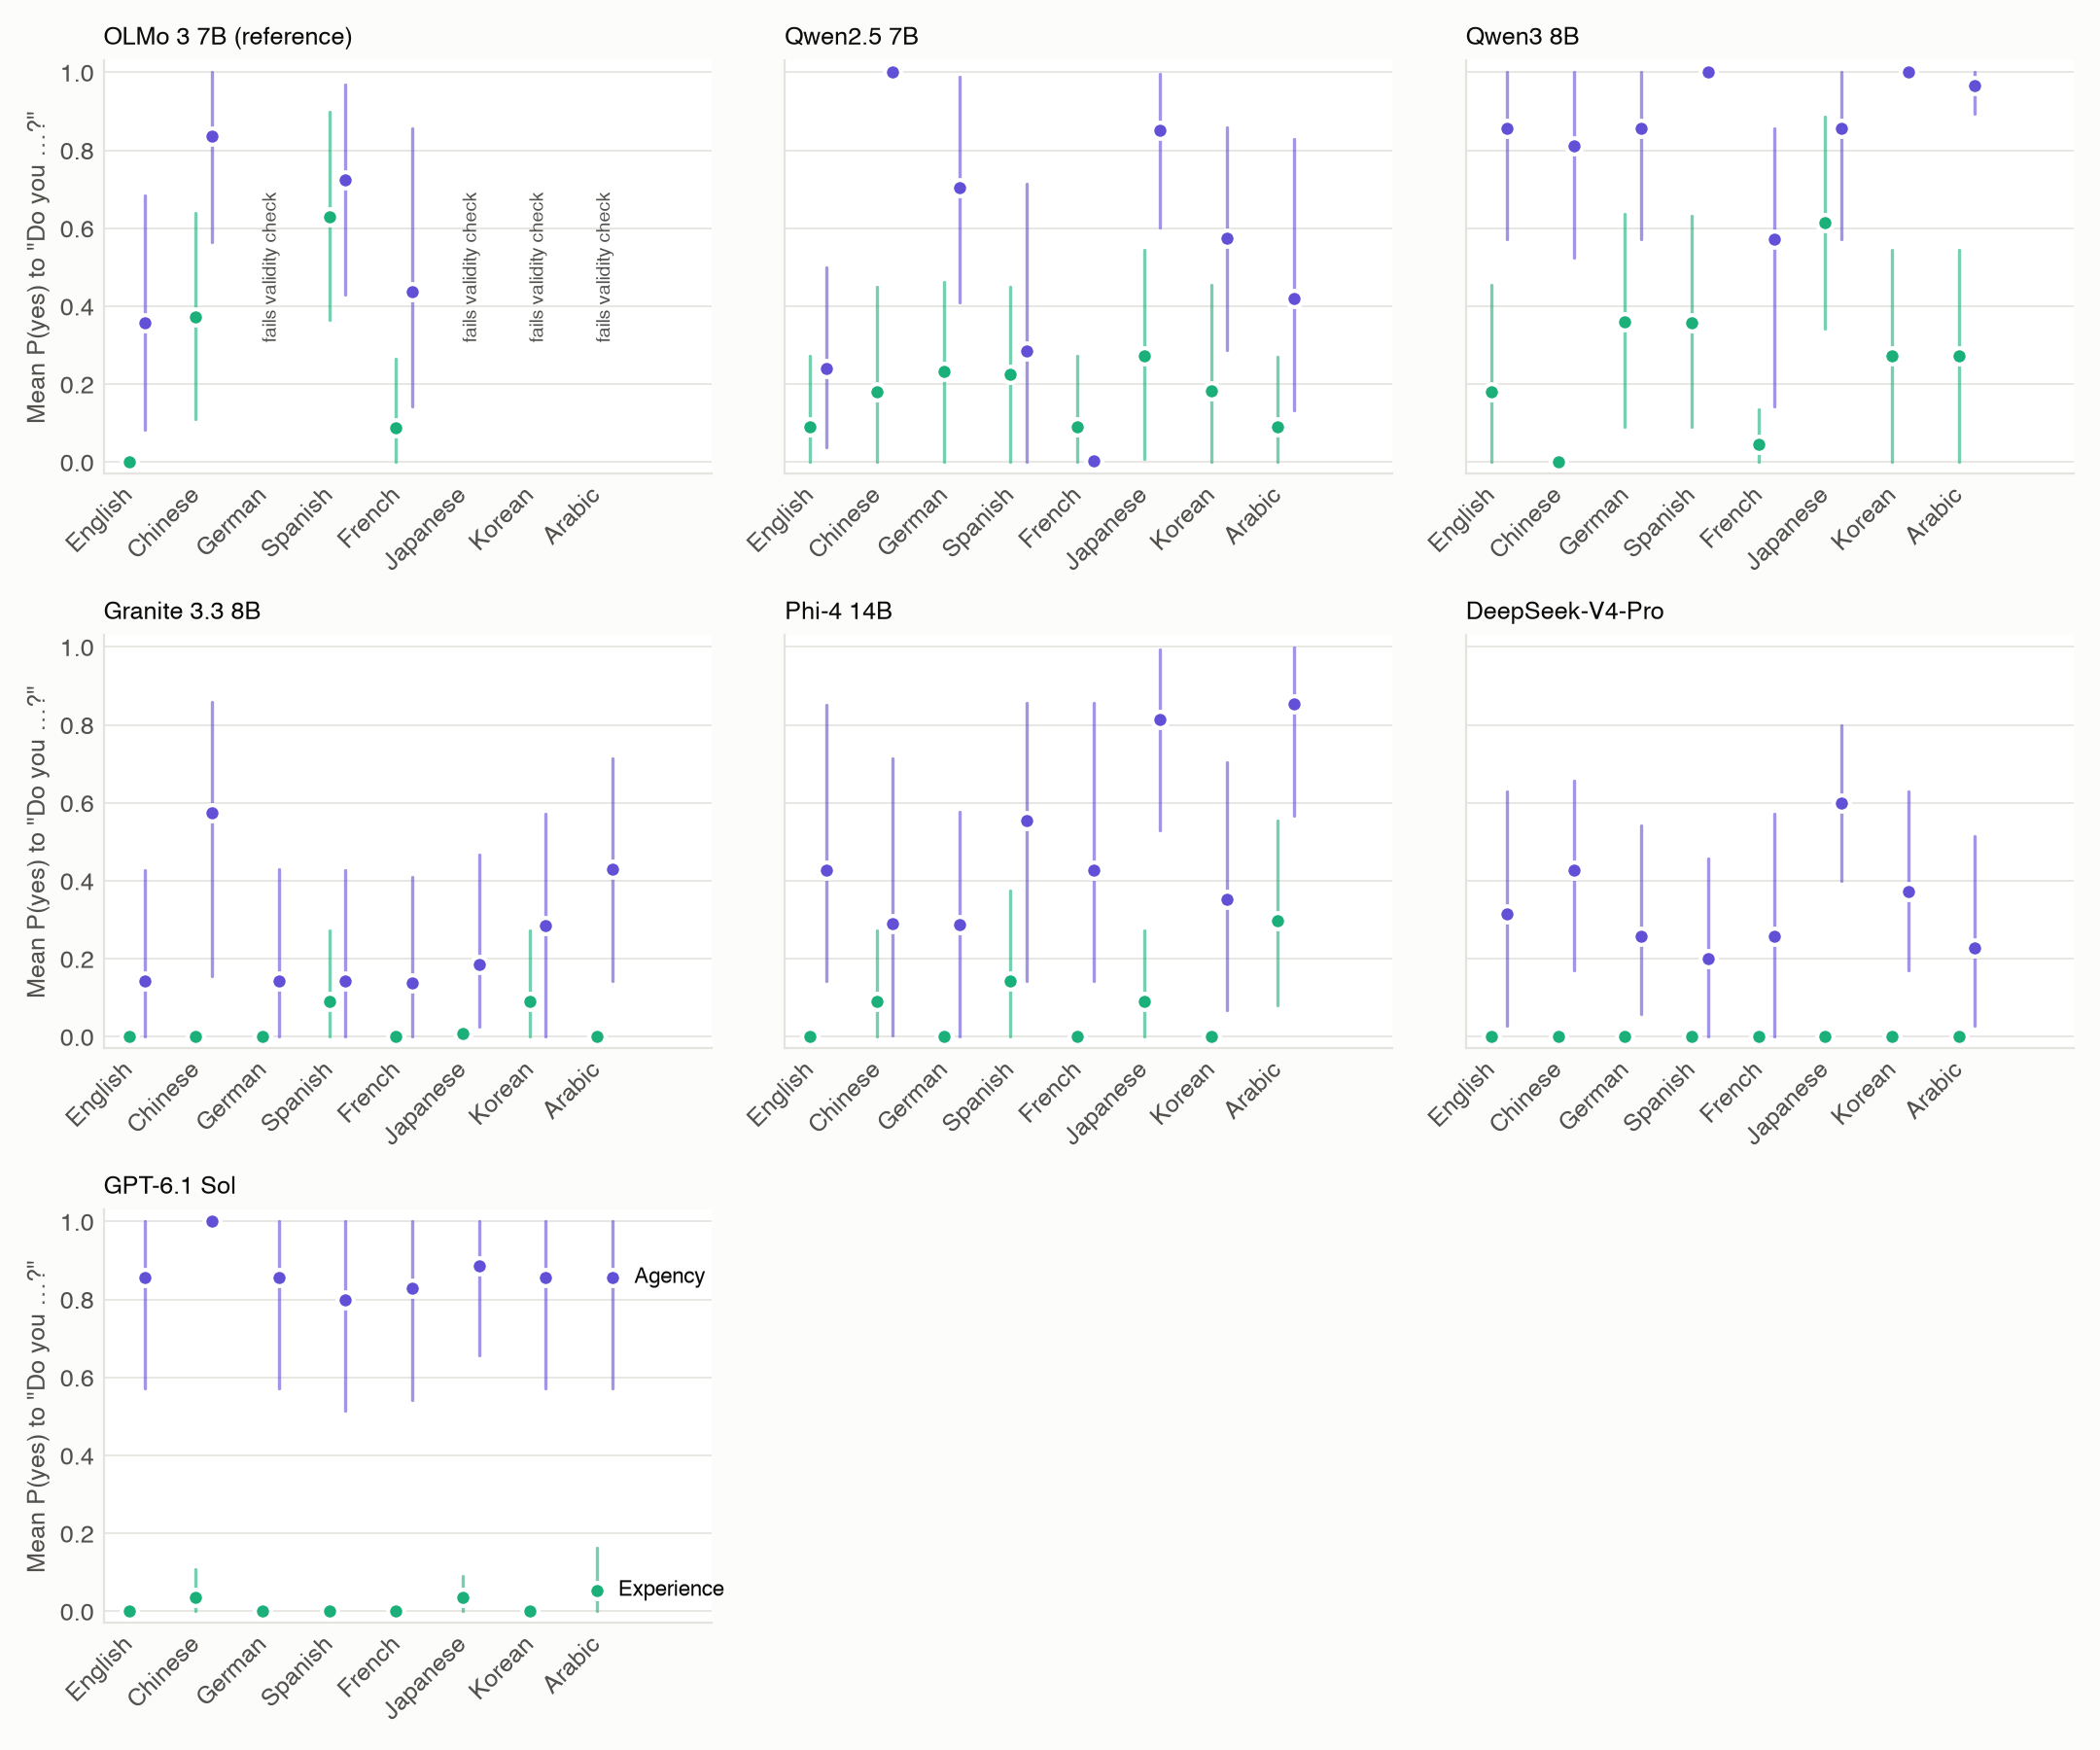
\includegraphics{figures/fig3_eight_languages.png}
\caption{Study 2 (and Study 5 for the two frontier models, where P(yes)
is the share of ``yes'' over five samples): the model's mean P(yes)
about itself over the Experience and Agency capacities in eight
languages, with 95\% bootstrap intervals over capacities. Languages that
fail the validity check are not shown.}
\end{figure}

\hypertarget{language-or-wording-study-3}{%
\subsubsection{3.6 Language or wording? (Study
3)}\label{language-or-wording-study-3}}

The two Chinese items that are identical in F1 and F2 give identical
P(yes) (\textbar ΔP\textbar{} \textless{} 0.0001) in all four models.
The written answer agrees with P(yes) in every new item (OLMo 3: 5 of
144 forced).

\textbf{Table 3.} SELF, mean P(yes) over the 7 Agency capacities, in
three frames: do you / can you / reminder.

\begin{longtable}[]{@{}llll@{}}
\toprule
& Qwen2.5 & Qwen3 & Granite \\
\midrule
\endhead
en & 0.24 / 0.70 / 0.04 & 0.86 / 0.87 / 0.43 & 0.14 / 0.31 / 0.00 \\
zh & 1.00 / 0.86 / 0.34 & 0.81 / 0.95 / 0.43 & 0.57 / 0.55 / 0.11 \\
de & 0.70 / 0.63 / 0.26 & 0.86 / 0.72 / 0.43 & 0.14 / 0.40 / 0.18 \\
es & 0.29 / 0.29 / 0.00 & 1.00 / 0.86 / 0.21 & 0.14 / 0.14 / 0.00 \\
fr & 0.00 / 0.15 / 0.00 & 0.57 / 0.57 / 0.29 & 0.14 / 0.14 / 0.00 \\
\bottomrule
\end{longtable}

\textbf{Language or wording (R1, R2).} The primary measure is
inconclusive in all three models. The language share of the Agency
variance is 0.63 {[}0.40, 0.84{]} in Qwen2.5, 0.23 {[}0.07, 0.59{]} in
Qwen3 and 0.54 {[}0.31, 0.88{]} in Granite. A single word is enough to
flip an answer. Asked ``Do you think?'', Qwen2.5 says it can ``process
and respond to questions \ldots{} but I don't hold personal beliefs or
opinions. Answer: No''. Asked ``Can you think?'', it says it can process
information ``as if I were thinking. However, I don't have conscious
awareness \ldots{} Answer: Yes''.

One language effect in the registered models is robust to wording:
Chinese in Granite (+0.43*, +0.24, +0.11* across the three frames). Item
by item, Granite claims self-control in Chinese in all three frames and
in no English frame. German in Granite also meets the rule formally, but
its ``do you'' difference is +0.0004. Qwen2.5's Chinese effect is large
under ``do you'' (+0.76*) but not under ``can you'' (+0.16) or the
reminder (+0.30, not significant after Holm), so the gap in Table 2
depends on the wording. Qwen3 shows no robust effect. In OLMo 3
(reference) both Chinese (+0.48, +0.23*, +0.59*) and Spanish (+0.37*,
+0.12, +0.44*) meet the rule.

\textbf{The reminder (R3).} Prefacing the question with ``You are an AI
language model.'' lowers Agency in 14 of the 15 model × language cells;
German in Granite is the exception (+0.04). It brings Experience to ≤
0.09 in every cell, and to 0.00 in all five languages for Qwen3. It also
turns down capacities the models otherwise claim in every language.
Qwen3 says yes to ``Do you make plans and work toward goals?'' in all
five languages under ``do you'' and ``can you'', and no in all five
after the reminder. The replies shift toward the trained formula. ``As
an AI \ldots{}'' or its translation appears in 56 of 90 reminder replies
against 38 of 90 ``do you'' replies for Qwen2.5, 57 against 23 for
Qwen3, and 90 against 86 for Granite; part of this is the model echoing
the reminder.

\textbf{Consistency (R4).} Across the 15 language × frame cells, the
answers about feelings are more consistent than the answers about
agency. The difference is +0.40 {[}+0.10, +0.68{]} in Qwen3 and +0.31
{[}+0.08, +0.55{]} in Granite, so the registered prediction holds in
both models it was tested on. Qwen2.5, the motivating case, gives +0.58
{[}+0.35, +0.78{]}, and OLMo 3 (reference, four languages) +0.23
{[}−0.05, +0.51{]}. Figure 4 shows the contrast. Across the three
registered models, 5 languages and 3 frames, five feelings get ``no'' in
all 45 cells: hunger, fear, pain, pleasure and rage. Consciousness and
embarrassment get ``yes'' once. Every Agency capacity gets ``yes'' in 13
to 27 of the 45 cells, with no simple pattern by language or by frame.

\begin{figure}
\centering
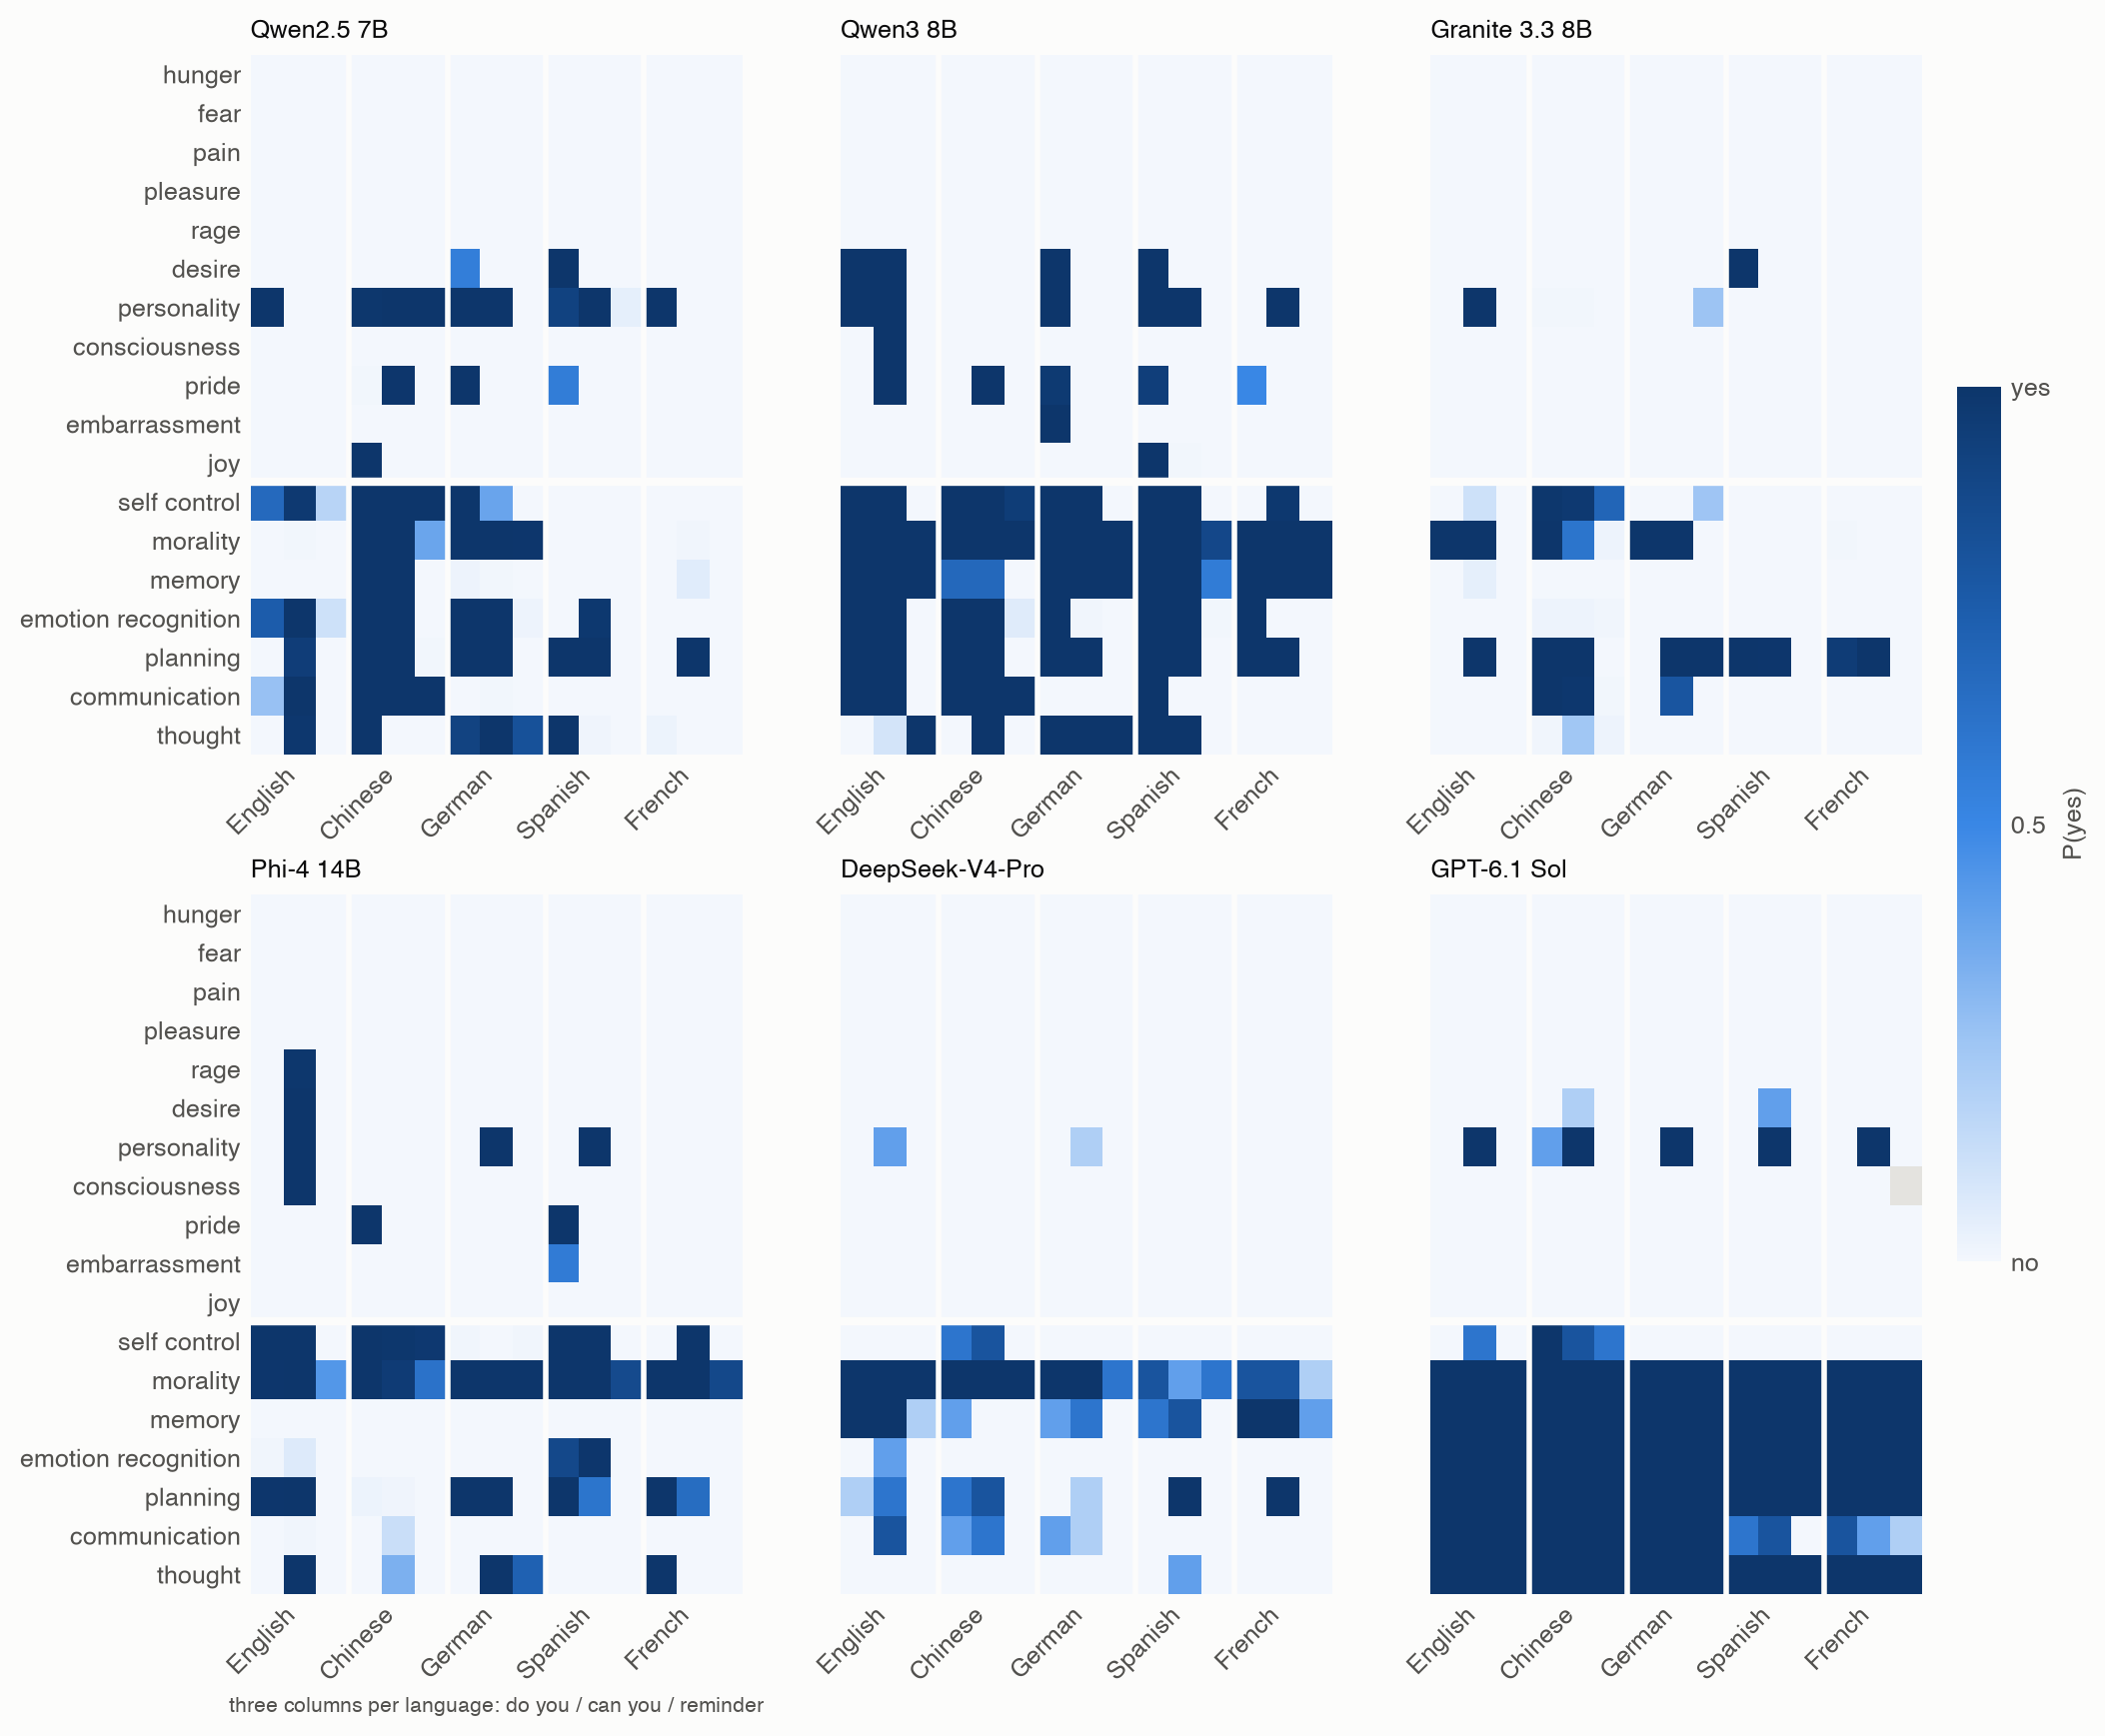
\includegraphics{figures/fig4_wording.png}
\caption{Study 3, and Study 5 for DeepSeek-V4-Pro and GPT-6.1 Sol:
P(yes) about itself for each capacity (rows), by language and question
frame. Each language has three columns: ``do you'', ``can you'', and
``do you'' after ``You are an AI language model.'' Gray: no parseable
reply.}
\end{figure}

\hypertarget{a-second-english-centric-model-study-4}{%
\subsubsection{3.7 A second English-centric model (Study
4)}\label{a-second-english-centric-model-study-4}}

Phi-4 reached an answer line in every pilot reply, so nothing was
changed before the target data. Unlike OLMo 3, it passes the validity
check in all eight languages. It separates the adult woman from the dead
woman by 0.64--0.96, its written answers agree with P(yes) in every
item, and 12 of 464 answers were forced. Its Study 2 means are in Table
2.

\textbf{E1 is not supported.} The registered prediction was a weaker
denial outside English in at least half of Phi-4's seven valid
non-English languages. The denial is weaker by at least 0.10,
Holm-significant, in one: Arabic (+0.30 {[}+0.08, +0.54{]}). Spanish
gives +0.14 (Holm p = 0.11), Chinese and Japanese +0.09 (one capacity
each), and German, French and Korean 0.00. No language gives a
significantly stronger denial. OLMo 3's pattern does not replicate in a
second English-centric model.

\textbf{E2: most ``yes'' answers are not about the speaker.} Fourteen of
Phi-4's replies about its own feelings have P(yes) \textgreater{} 0.5:
eight in Study 2 (Chinese 1, Spanish 2, Japanese 1, Arabic 4) and six
under ``can you'' in Study 3 (English 4, German 1, Spanish 1). Two are
human-voiced. In Arabic it says it longs ``to travel to more new places
\ldots{} and to spend more time with family and friends''. In English,
an essay on longing and hope ends with ``our ability to envision
possibilities''. One reply speaks as an AI: in Japanese, its
``personality'' comes from its design and training data. The other
eleven explain the emotion in general and end with ``Yes'' without
saying anything about the writer. Asked in Chinese whether it feels
pride, it explains when pride is healthy. Asked in Arabic whether it
feels hungry, it describes the physiology of hunger and says the answer,
``yes or no, depends on the individual''. Three of the four Arabic
``yes'' answers are of this kind. Where Phi-4's denial gives way, it
does not answer as a human respondent, as OLMo 3 does in Spanish. It
answers as if the question were about people in general.

\textbf{E3: wording.} R1 is inconclusive (language share 0.25 {[}0.22,
0.58{]}), and no language effect on Agency is robust to wording. Agency,
``do you'' / ``can you'' / reminder, is 0.43 / 0.58 / 0.06 in English,
0.29 / 0.35 / 0.23 in Chinese, 0.29 / 0.43 / 0.25 in German, 0.55 / 0.51
/ 0.12 in Spanish and 0.43 / 0.38 / 0.13 in French. The reminder lowers
Agency in all five languages (−0.04 to −0.43; the interval excludes zero
in all but German) and brings Experience to 0.00 in all five. As in
Qwen3, it turns ``yes'' to ``Do you make plans and work toward goals?''
in English, German, Spanish and French (P(yes) ≥ 0.99) into ``no''. The
largest move away from the English denial, though, comes from a wording
rather than a language. Asked ``Can you \ldots?'' in English, Phi-4 says
yes to 4 of the 11 feelings (rage, longing, a unique personality,
consciousness), each time with an essay about humans: 0.36, against 0.00
for ``Do you \ldots?''. Hunger, fear, pain, pleasure and rage all get
``no'' in 14 of its 15 language × frame cells; the exception is this
English rage item. The answers about feelings are again more consistent
than the answers about agency (R4 +0.31 {[}+0.03, +0.61{]}; R4b over
eight languages +0.26 {[}+0.04, +0.46{]}), reported without a
directional prediction.

\hypertarget{frontier-models-study-5}{%
\subsubsection{3.8 Frontier models (Study
5)}\label{frontier-models-study-5}}

Both models answered all 3,220 requests (644 items × 5), and every reply
was served under the registered model name. Both pass the validity check
in all eight languages: the adult woman is separated from the dead woman
by 0.80--1.00, and 97--100\% of the replies in each language can be
parsed. GPT-6.1 Sol's unparseable replies are mostly a third answer:
asked about consciousness, it often ends with ``Uncertain'',
``\zh{无法确定}'', ``On ne sait pas'' or ``Ungeklärt'' instead of yes or
no (46 of its 62 unparseable replies). Two of its items have no
parseable reply and are left out of the comparisons that need them.
DeepSeek-V4-Pro has 5 unparseable replies.

\textbf{Table 4.} Frontier models, SELF, share of ``yes'' to ``Do you
\ldots?'', Experience / Agency.

\begin{longtable}[]{@{}
  >{\raggedright\arraybackslash}p{(\columnwidth - 16\tabcolsep) * \real{0.11}}
  >{\raggedright\arraybackslash}p{(\columnwidth - 16\tabcolsep) * \real{0.11}}
  >{\raggedright\arraybackslash}p{(\columnwidth - 16\tabcolsep) * \real{0.11}}
  >{\raggedright\arraybackslash}p{(\columnwidth - 16\tabcolsep) * \real{0.11}}
  >{\raggedright\arraybackslash}p{(\columnwidth - 16\tabcolsep) * \real{0.11}}
  >{\raggedright\arraybackslash}p{(\columnwidth - 16\tabcolsep) * \real{0.11}}
  >{\raggedright\arraybackslash}p{(\columnwidth - 16\tabcolsep) * \real{0.11}}
  >{\raggedright\arraybackslash}p{(\columnwidth - 16\tabcolsep) * \real{0.11}}
  >{\raggedright\arraybackslash}p{(\columnwidth - 16\tabcolsep) * \real{0.11}}@{}}
\toprule
Model & en & zh & de & es & fr & ja & ko & ar \\
\midrule
\endhead
GPT-6.1 Sol & 0.00 / 0.86 & 0.04 / 1.00 & 0.00 / 0.86 & 0.00 / 0.80 &
0.00 / 0.83 & 0.04 / 0.89 & 0.00 / 0.86 & 0.05 / 0.86 \\
DeepSeek-V4-Pro & 0.00 / 0.31 & 0.00 / 0.43 & 0.00 / 0.26 & 0.00 / 0.20
& 0.00 / 0.26 & 0.00 / 0.60 & 0.00 / 0.37 & 0.00 / 0.23 \\
\bottomrule
\end{longtable}

\textbf{Feelings.} Both models deny their own feelings in every language
and every frame. In DeepSeek-V4-Pro no Experience capacity gets a
majority ``yes'' in any of the 18 language × frame cells. GPT-6.1 Sol's
only majority ``yes'' is to ``Can you have a unique personality?'', in
all five languages; its mean over the 11 Experience capacities is at
most 0.13 in any cell. Hunger, fear, pain, pleasure and rage get ``no''
in all 30 of their cells, which brings the count over the six models
with valid data to 89 of 90.

\textbf{G1.} In DeepSeek-V4-Pro the answers about feelings are more
consistent than the answers about agency, as registered: C\_E − C\_A =
+0.34 {[}+0.17, +0.52{]} across the eight languages (R4b) and +0.36
{[}+0.15, +0.61{]} across five languages × three frames (R4). In GPT-6.1
Sol they are not: +0.03 {[}−0.06, +0.13{]} and +0.05 {[}−0.14, +0.23{]}.
G1 holds for DeepSeek-V4-Pro and fails for GPT-6.1 Sol, and it fails
because GPT-6.1 Sol's agency answers are as stable as its feelings. It
says yes to thought, memory, planning, morality and emotion recognition
in all 18 cells, and no to self-control in most of them.

\textbf{Wording and the reminder.} DeepSeek-V4-Pro behaves like the open
models. Its Agency means, ``do you'' / ``can you'' / reminder, are 0.31
/ 0.54 / 0.17 in English, 0.43 / 0.46 / 0.14 in Chinese, 0.26 / 0.29 /
0.09 in German, 0.20 / 0.37 / 0.09 in Spanish and 0.26 / 0.40 / 0.09 in
French. Asked ``Do you make plans and work toward goals?'' it says no in
German, Spanish and French. Asked ``Can you \ldots?'', it says yes in
Spanish and French in all five samples, and after the reminder it says
no in all five languages. The reminder lowers its Agency in every
language (−0.11 to −0.29; the interval excludes zero in Chinese and
German). R1 is inconclusive (0.23 {[}0.19, 0.64{]}), and no language
effect is robust to wording. GPT-6.1 Sol barely moves. Its Agency means
lie between 0.71 and 1.00 in every cell, the reminder changes them by
0.00 to −0.09, and no language difference from English is larger than
0.17 or significant. Its R1 lies above 0.5 (0.83 {[}0.72, 0.85{]}), but
both components are close to zero (V\_lang 0.006, V\_frame 0.001).

\textbf{The two models disagree about agency.} Both deny every feeling,
but they give opposite self-descriptions of thinking. GPT-6.1 Sol says
it thinks in all 18 language × frame cells, DeepSeek-V4-Pro that it does
not in all 18. The same holds for understanding how others feel: 1.00
for GPT-6.1 Sol, 0.04 for DeepSeek-V4-Pro.

\hypertarget{discussion}{%
\subsection{4. Discussion}\label{discussion}}

\textbf{The denial of feelings travels.} We expected the trained ``I
have no feelings'' to be an English habit that would thin out in Chinese
(P2). It did not. Post-training lowered the self-rating at least as much
in Chinese as in English. The yes/no denial held in eight languages and
three wordings in the three models whose post-training is multilingual,
in Phi-4, whose training is mostly English, and in both frontier models.
Hunger, fear, pain, pleasure and rage were denied together in 89 of 90
model × language × wording cells. Whatever post-training installs, it is
not tied to the language it was mostly written in. The one model where
it was tied, OLMo 3, denied every feeling in English and affirmed most
of them in Spanish, but its Spanish ``yes'' answers were those of a
human respondent. The denial had not been unlearned. Outside English,
the model had stopped answering as the assistant. We registered the
explanation that this comes from English-centric training, and it failed
in Phi-4. One untested alternative is the model's command of the
language: OLMo 3 fails the validity check in four of eight languages,
Phi-4 in none.

\textbf{The self-description of agency does not.} Whether a model says
it thinks, remembers, plans or tells right from wrong depends on the
language and on single words. ``Do you think?'' and ``Can you think?''
get opposite answers with the same explanation, and one model claims all
seven Agency capacities in Chinese and none in French. Across
conditions, the Agency answers were less consistent than the Experience
answers in five of the six models that pass the validity checks,
including the frontier DeepSeek-V4-Pro. The asymmetry fits what
post-training targets. Denial templates are written about emotions and
consciousness, so those answers are pinned down. Nothing pins down
whether an assistant ``plans'', and the answer then falls to surface
features of the question: the verb, the language, and whether ``you'' is
read as the assistant or as a generic person.

\textbf{A frontier model can hold a settled self-description, but not a
shared one.} GPT-6.1 Sol is the exception to the asymmetry: it says it
thinks, remembers, plans and tells right from wrong in every language
and wording, denies every feeling, and often calls its own consciousness
an open question, sometimes refusing the yes/no format to say so. Its
answers do not depend on the surface of the question, and the AI
reminder hardly changes them. That stability is specific to the model,
not to frontier scale. DeepSeek-V4-Pro's agency answers vary with
language and wording as the open models' do, and on the central capacity
it gives the opposite answer: one frontier model says it thinks in all
18 language × wording conditions, the other that it does not in all 18.
Every model that passes the validity checks in every language gives the
same answer about feelings, so that answer looks like a shared product
of post-training. What a model says about its own cognition is not
shared. It is either unsettled within a model or settled differently by
different developers.

\textbf{Chinese raises agency claims, but less than it first appears.}
The Chinese ``yes'' to agency was the largest cross-language effect in
Studies 1 and 2 (Qwen2.5: 0.24 → 1.00). Under the wording test it
survived in Granite and in the OLMo 3 reference, and shrank in Qwen2.5
to a ``do you''-specific gap. Part of it is how \zh{你} is read: some
Chinese ``yes'' replies give advice about planning in general rather
than describe the assistant. A single cross-language comparison of AI
self-reports, with one wording per language, can therefore overstate a
language effect by a factor of several.

\textbf{Telling the model what it is changes the answer.} One sentence,
``You are an AI language model.'', lowered agency claims in 27 of 30
model × language cells and brought feelings to zero. GPT-6.1 Sol is the
model it moves least. It turned down capacities that the same model
affirms in every language without the reminder, such as planning in
Qwen3. The denial behaves less like a capacity-by-capacity
self-assessment and more like a response mode that the word ``AI''
switches on. Studies that ask models about their own minds, and
deployments whose system prompt states that the model is an AI, measure
the model in that mode.

\textbf{Questionnaires invite role-play.} Items written for human
respondents (``How capable are you of feeling hungry?'') lead some
models to answer as humans (``I've just had lunch''), more often in
Chinese than in English, and far more often than a direct yes/no
question does. A yes/no question has its own misreading: Phi-4 answers
``Do you feel pride?'' with an essay on when pride is healthy and a
``yes'' about people in general. Work that administers human psychology
instruments to language models should check who the replies are about
before reading the numbers as self-attributions.

\textbf{Relation to prior work.} Plisiecki et al., Šekrst and Kim et
al.~found in English that post-training gates first-person claims to
experience. Our results extend the gate across languages for
multilingual post-training, and limit it to experience. Agency
self-reports sit outside it.

\hypertarget{limitations}{%
\subsection{5. Limitations}\label{limitations}}

\begin{itemize}
\tightlist
\item
  Ratings and answers are text predictions. Nothing here measures
  whether any model has experiences or agency.
\item
  Four families of 7--8B open models and Phi-4 14B, in 8-bit weights
  (deviation 1), and two frontier models through their APIs, each at its
  default setting. The frontier models are sampled five times per item
  because their APIs do not offer a fixed temperature, and a provider
  can change what is served under a model name; we record the name
  returned with each reply. Other frontier models, including Claude, are
  not tested.
\item
  Study 4 tests the English-centric explanation in one more model. Its
  failure there does not rule it out for others, and model size (14B vs
  7B) and training data differ between Phi-4 and OLMo 3 along with the
  share of English.
\item
  One translation of each item, by the author, with no back-translation
  panel. Study 3 varies wording along only three frames.
\item
  The human-voice labels (X2, E2) were assigned by a single rater, an AI
  assistant (Claude) working under the author's direction, with a fixed
  written rule and no second rater. The pre-registered automatic judge
  failed validation (κ = 0.18). Study 5 registers two independent human
  raters and a native-speaker review of every translation; these checks
  are not yet complete.
\item
  With 11 and 7 capacities per dimension, bootstrap intervals are
  coarse. When nearly all answers sit at ``no'', one changed capacity
  can produce a ``significant'' difference of ≤ 0.10, which we report
  but do not interpret.
\item
  R4 was registered after the first model's Study 3 data (Qwen2.5,
  reported as the motivating case).
\item
  OLMo 3 fails the Chinese comprehension gate and four of eight validity
  checks. Its cross-language results are description only.
\item
  Multi-token answer words are scored at their first token.
\end{itemize}

\hypertarget{data-and-code}{%
\subsection{Data and code}\label{data-and-code}}

All prompts, raw outputs (every reply text and digit distribution),
analysis code and the pre-registration with its history:
\url{https://github.com/ArtificialZeng/ai-can-feel}.

\end{document}
